\section{Probabilidade de Erro: \texorpdfstring{$M$}{M}-QAM}
Para calcular a probabilidade de erro $P(e)$ de cada constelação~\ref{eq:Pe_M_QAM} é necessário computar a energia da cosnstelação e do ruído, respectivamente, $E_s$ e $N_o$, que é desenvolvida em~\cite{Cecilio}. A função~\href{https://raw.githubusercontent.com/lucasabdalah/Courses-HWs/SCD/Sistemas%20de%20Comunicacoes%20Digitais/matlab/problema2/Pe_MQAM.m}{\colorbox{gray!20}{\color{red}Pe\_MQAM.m}} é utlizada para calcular a probabilidade de erro.
\begin{equation}
    P(e) = 4 \left(1-\frac{1}{\sqrt{M}}\right) Q\left(\sqrt{\frac{3}{M-1}\frac{E_s}{N_0}}\right) - 4\left(1-\frac{1}{\sqrt{M}}\right)^2 Q^2\left(\sqrt{\frac{3}{M-1}\frac{E_s}{N_0}}\right)
    \label{eq:Pe_M_QAM}
\end{equation}

Para valores mais elevados de relação sinal-ruído(\textit{SNR}), a equação~\ref{eq:Pe_M_QAM} pode ser reduzida para~\ref{eq:Pe_reduzida_M_QAM}, pois o segundo termo ao quadrado se torna irrelevante.
\begin{equation}
    P(e) = 4 \left(1-\frac{1}{\sqrt{M}}\right) Q\left(\sqrt{\frac{3}{M-1}\frac{E_s}{N_0}}\right)
    \label{eq:Pe_reduzida_M_QAM}
\end{equation}

\begin{figure}[!ht]
    \centering
    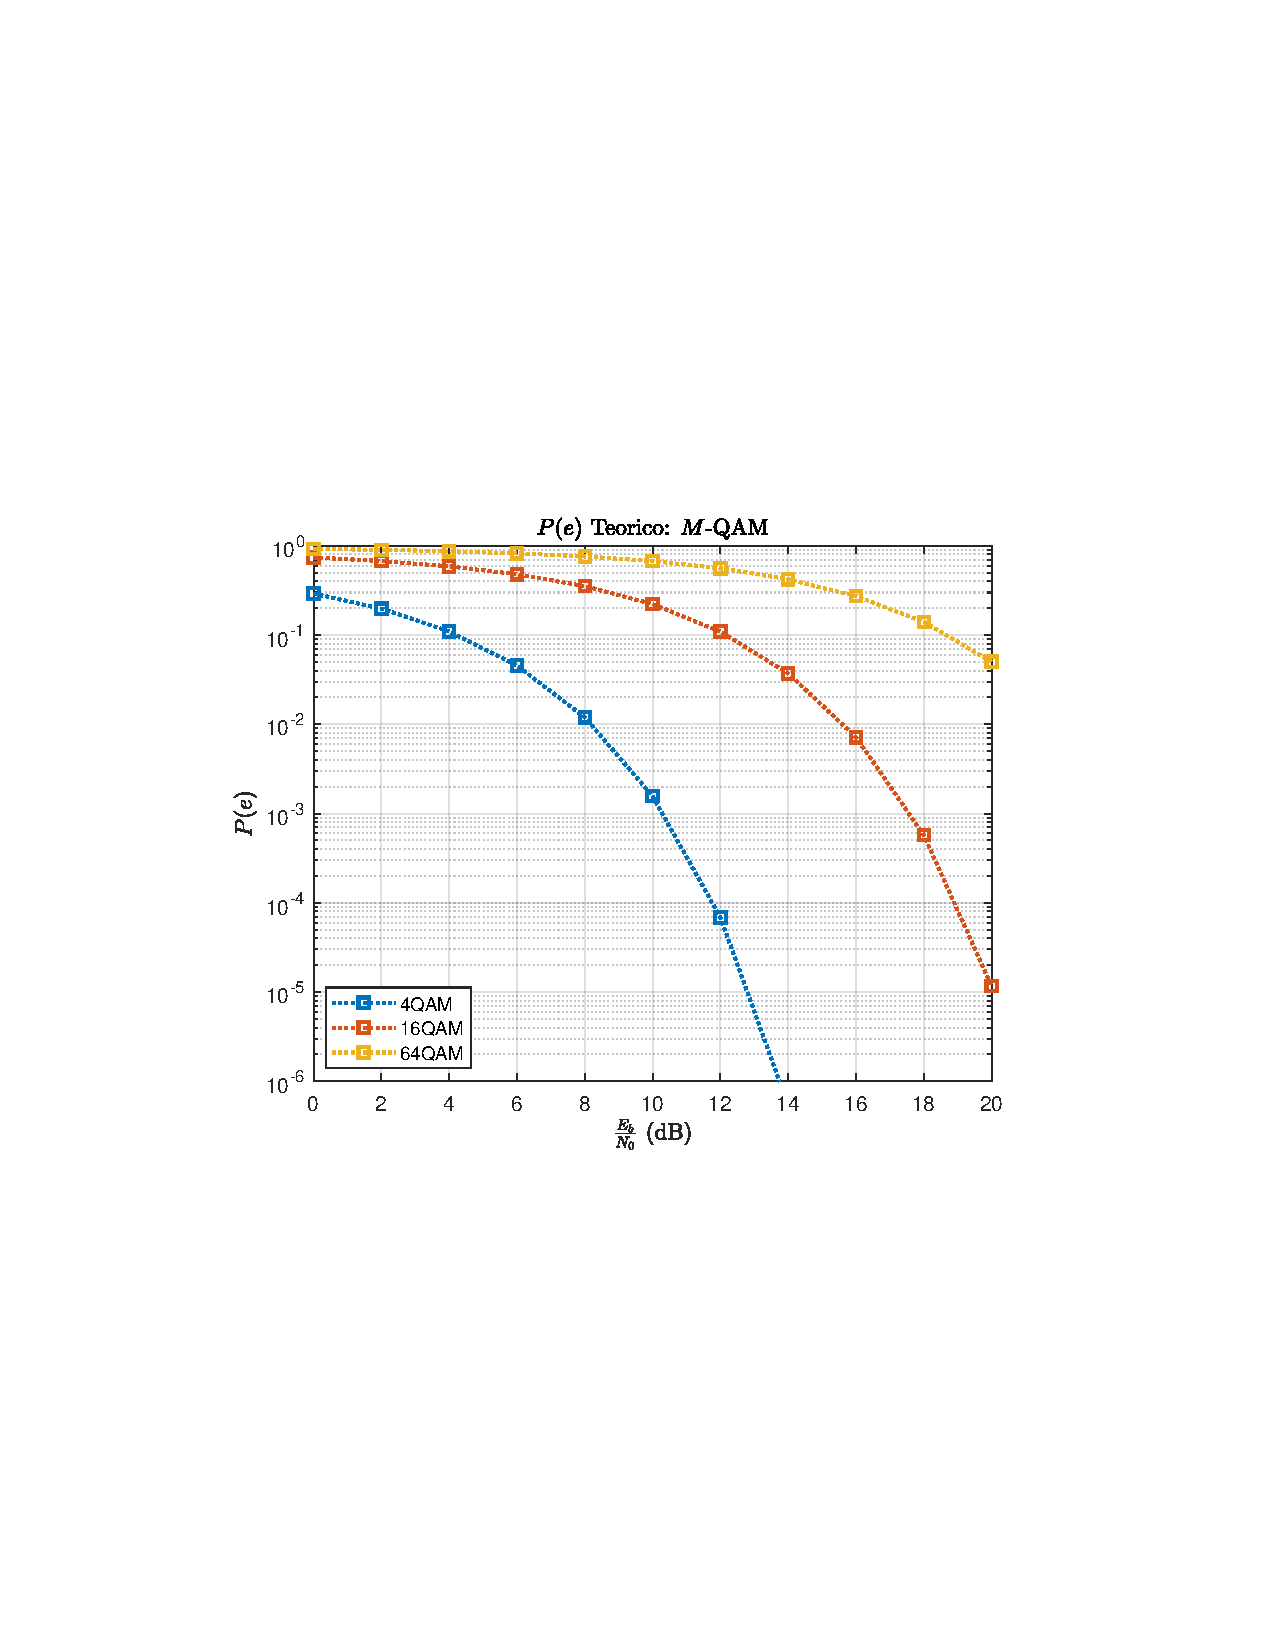
\includegraphics[width=1.0\textwidth,clip=true,trim={1.5cm 8.5cm 1.8cm 8.3cm}]{C:/Users/lukin/Documents/GitHub/Courses-HWs/Sistemas de Comunicacoes Digitais/matlab/problema2/fig/Erro_Teorico_MQAM.pdf}
    \caption{Probabilidade de erro $(P(e))$ teórico $M$-QAM.}
    \label{fig:Erro_Teorico_MQAM}
\end{figure}

Nas simulações realizadas, os resultados são semelhantes, além de reduzir o custo computacional.

Entretanto, para manter uma fidedignidade númerico aos resultados, o gráfico mostrado na figura~\ref{fig:Erro_Teorico_MQAM} a probabilidade $P(e)$ é caculada a partir da equação completa~\ref{eq:Pe_M_QAM}, variando a \textit{SNR} de 0:2:20 dB.